\documentclass[aspectratio=169]{beamer}

\usepackage[utf8]{inputenc}
\usepackage[T1]{fontenc}
\usepackage[brazil]{babel}
\usepackage{ubuntu}
\usepackage{nameref}
\usepackage{hyperref}
\usepackage{courier}

\usetheme{Ampang}
\usecolortheme{ampangcolor}

%Custom title page
\defbeamertemplate*{title page}{customized}[1][]{
  \centering
  \vfill
  \usebeamercolor[fg]{titlegraphic}\inserttitlegraphic\par
  \vskip2em\par
  \usebeamercolor{author}\centerline{\insertauthor}\par
  \usebeamerfont{date}\centerline{\insertdate}
}

%Macro to get section title
\makeatletter
\newcommand*{\currentname}{\@currentlabelname}
\makeatother

%Title page setup
\titlegraphic{
\includegraphics[width=\textwidth]{img/Git-logo.png}}
\author{Pedro Castilho}
\date{\today}

%Create section titles whenever we start a section
\AtBeginSection[]{
  \begin{frame}
    \vfill
    \begin{center}
      \Huge \currentname
    \end{center}
    \vfill
  \end{frame}
}

%Finished setting up stuff, start the actual document
\begin{document}

\begin{frame}
  \titlepage
\end{frame}

\section{Introdução}
\subsection{O que é Git?}
\begin{frame}
  \frametitle{\currentname}
  \begin{itemize}
    \uncover<1->{\item Sistema de versionamento}
    \uncover<2->{\item Distribuído}
    \uncover<3->{\item Livre e de código aberto}
  \end{itemize}
  \begin{center}
    \uncover<4->{
\includegraphics[height=0.3\textheight]{img/Its-free.jpg}}
  \end{center}
\end{frame}

\subsection{Por que usar Git?}
\begin{frame}
  \frametitle{\currentname}
  \begin{center}
    \uncover<2->{\Huge O que acontece quando você \textit{não} usa git:}
  \end{center}
\end{frame}

\begin{frame}
  \frametitle{\currentname}
  \begin{center}
    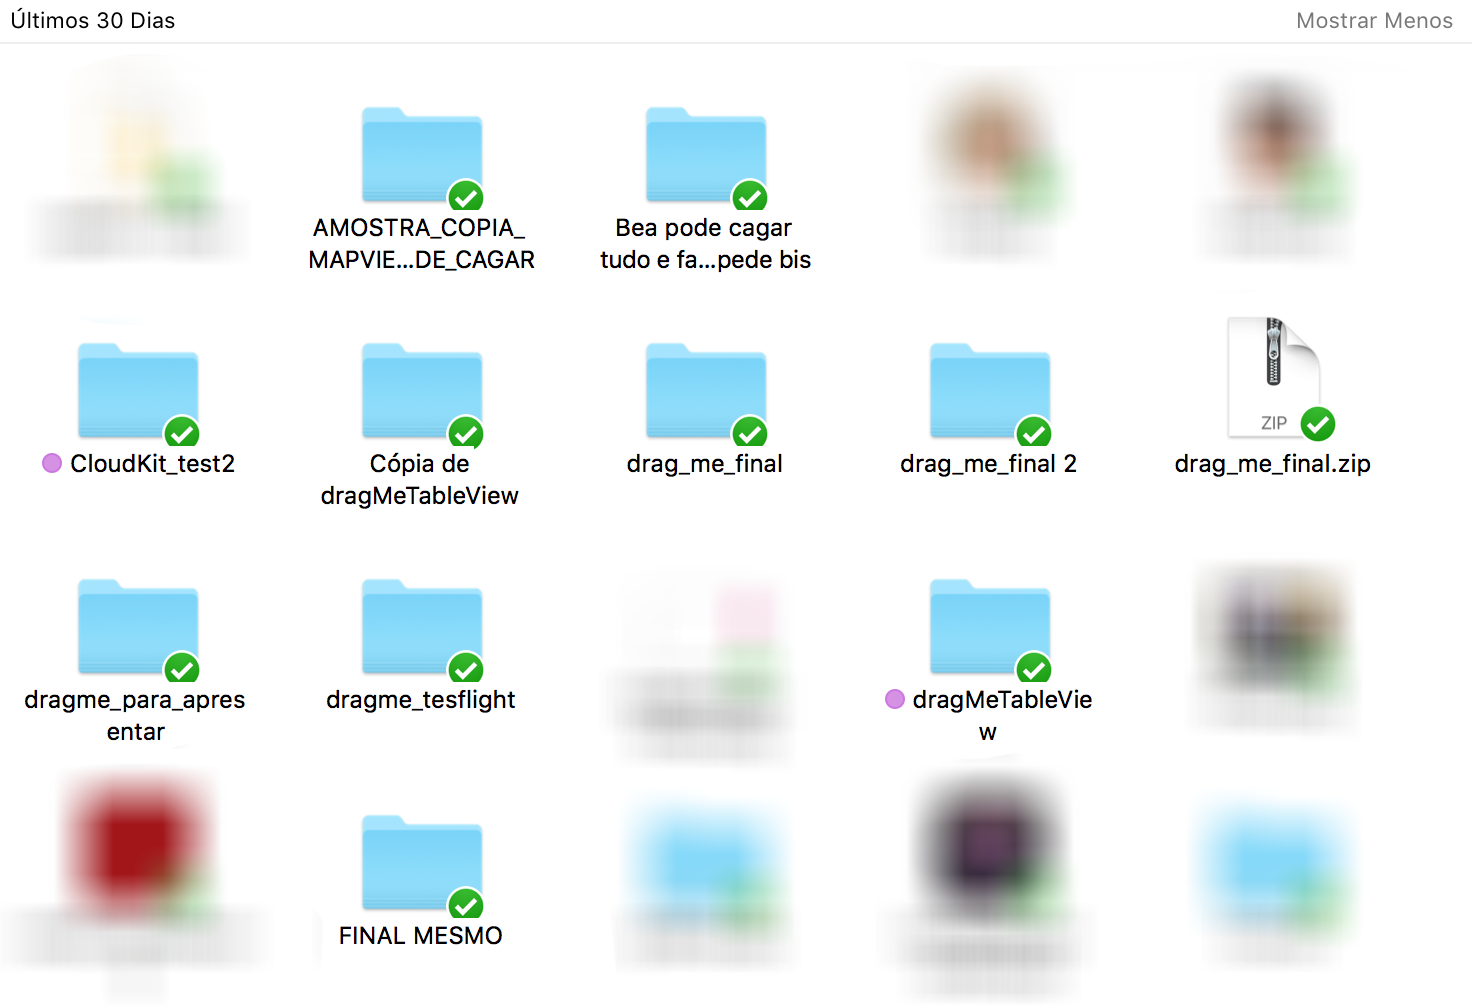
\includegraphics[height=0.8\textheight]{img/sem-git.png}
  \end{center}
\end{frame}

\begin{frame}
  \frametitle{\currentname}
  \begin{center}
    {\Huge O que acontece quando você \textit{usa} git:}
  \end{center}
\end{frame}

\begin{frame}
  \frametitle{\currentname}
  \begin{center}
    
\includegraphics[height=0.8\textheight]{img/com-git.jpg}
  \end{center}
\end{frame}

\subsection{Como usar Git?}
\begin{frame}
  \frametitle{\currentname}
  \begin{center}
    \uncover<2->{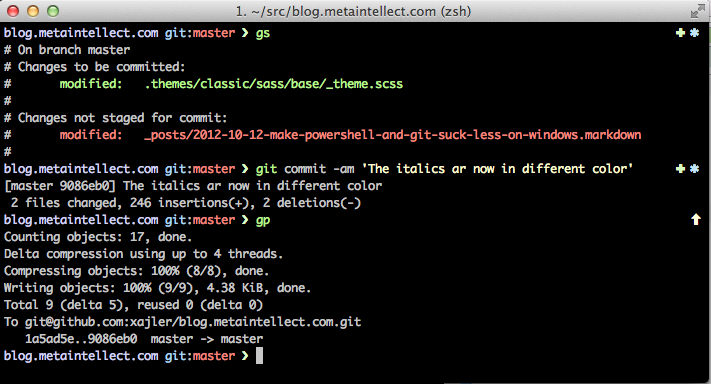
\includegraphics[height=0.6\textheight]{img/git-terminal.png}}
  \end{center}
\end{frame}

\begin{frame}
  \frametitle{\currentname}
  \begin{itemize}
    \uncover<1->{\item git foi pensado como programa de linha de comando}
    \uncover<2->{\item só na linha de comando todas as opções estão disponíveis}
    \uncover<3->{\item \alert<3>{existem} interfaces gráficas}
    \uncover<4->{\item (vou citar algumas no final)}
  \end{itemize}
\end{frame}

\subsection{Um aviso}
\begin{frame}
  \frametitle{\currentname}
  \begin{center}
    \uncover<2->{
\includegraphics[height=0.5\textheight]{img/dont-panic.png}}
  \end{center}
\end{frame}

\subsection{Baixando o Git}
\begin{frame}
  \frametitle{\currentname}
  \begin{center}
    \uncover<2->{\Huge Se você tem o Xcode, você tem git!}
  \end{center}
\end{frame}


\begin{frame}
  \frametitle{\currentname}
  \begin{itemize}
    \item Abra o terminal (Command + Espaço, escreva ``terminal'', Enter)
    \item Digite \texttt{git -{}-version}
  \end{itemize}
\end{frame}

\subsection{Atualizando o Git}
\begin{frame}
  \frametitle{\currentname}
  \vfill
  \begin{center}
    {\Huge Pergunte-me como!}
    \vskip2em 
    (Dica: é usando o Homebrew)
  \end{center}
  \vfill
\end{frame}

\subsection{git help}
\begin{frame}
  \frametitle{\currentname}
  \begin{itemize}
    \uncover<1->{\item O git contém ajuda para todos os comandos.}
    \uncover<2->{\item Digite \texttt{git help} para ver a lista.}
    \uncover<3->{\item (Lembre-se, não entre em pânico)}
    \uncover<4->{\item Ajuda de comandos específicos:}
    \uncover<5->{\item Digite \texttt{git help config}}
    \uncover<6->{\item Digite \texttt{q} para sair da ajuda.}
  \end{itemize}
\end{frame}

\section{Configurando o Git}
\subsection{git config}
\begin{frame}
  \frametitle{\currentname}
  \begin{itemize}
    \uncover<1->{\item Vamos começar configurando seu usuário no git.}
    \uncover<2->{\item Digite o seguinte no terminal:}
    \uncover<3->{\item \texttt{git config user.name ``Seu nome''}}
    \uncover<4->{\item \texttt{git config user.email \href{mailto:seu_email@provedor.com}{\nolinkurl{seu_email@provedor.com}}}}
    \uncover<5->{\item Agora digite \texttt{git config -{}-list}}
  \end{itemize}
\end{frame}

\begin{frame}
  \begin{center}
    {\Huge Dúvidas?}
  \end{center}
\end{frame}

\section{Trabalhando com repositório local}
\subsection{Working directory, Staging area, e Repositório}
\begin{frame}
  \frametitle{\currentname}
  \begin{center}
    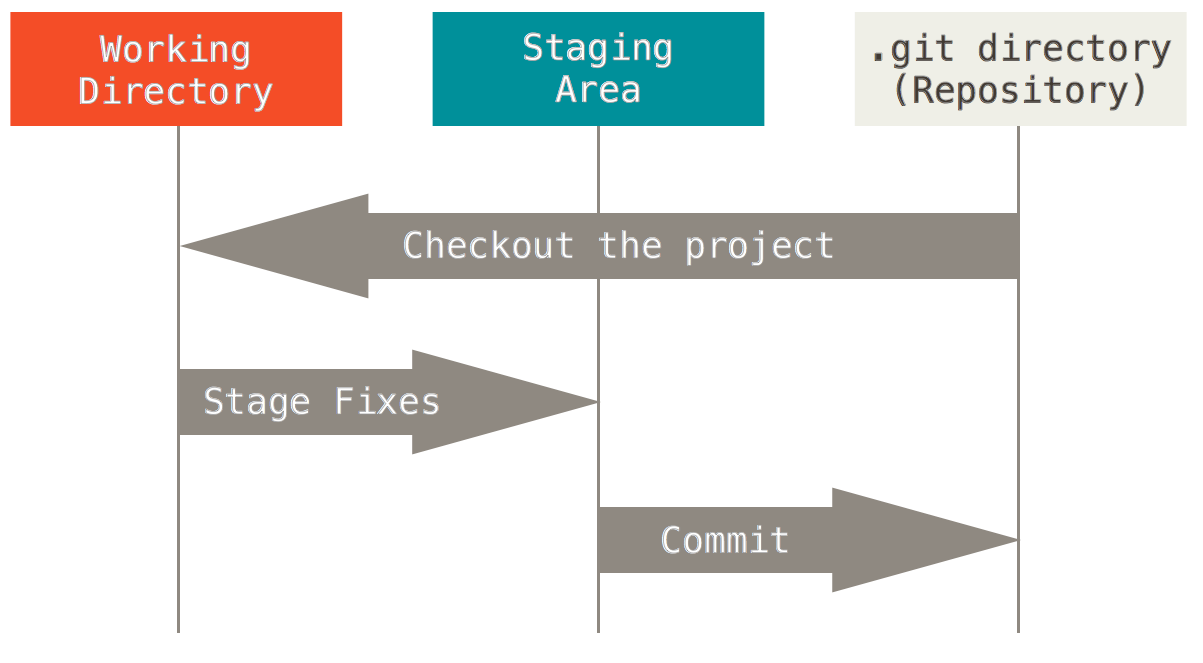
\includegraphics[height=0.5\textheight]{img/areas.png}
  \end{center}
\end{frame}

\subsection{git init}
\begin{frame}
  \frametitle{\currentname}
  \begin{itemize}
    \uncover<1->{\item Crie um novo projeto do Xcode (ou use a pasta de um projeto velho)}
    \uncover<2->{\item No terminal, vá para a pasta do projeto}
    \uncover<3->{\item Na pasta do projeto, digite \texttt{git init}}
    \uncover<4->{\item Se tudo der certo, agora você tem um repositório nessa pasta!}
  \end{itemize}
\end{frame}

\begin{frame}
  \frametitle{\currentname}
  \begin{center}
    {\Huge git init: cria um novo repositório}
  \end{center}
\end{frame}

\subsection{git status}
\begin{frame}
  \frametitle{\currentname}
  \begin{itemize}
    \uncover<1->{\item Na mesma pasta, digite \texttt{git status}}
    \uncover<2->{\item Deve surgir uma lista com vários ``Untracked files''}
    \uncover<3->{\item Esses arquivos estão no ``Working Directory''}
    \uncover<4->{\item Vamos colocá-los na ``Staging Area''.}
  \end{itemize}
\end{frame}

\begin{frame}
  \frametitle{\currentname}
  \begin{center}
    {\Huge git status: mostra o estado atual do ``Working Directory'' e da ``Staging Area''.}
  \end{center}
\end{frame}

%\subsection{git add}
\begin{frame}
  \frametitle{\currentname}
  \begin{itemize}
    \uncover<1->{\item Ainda na mesma pasta, escolha um arquivo da lista.}
    \uncover<2->{\item Digite \texttt{git add nome\_do\_arquivo}}
    \uncover<3->{\item Digite \texttt{git status} novamente.}
    \uncover<4->{\item O arquivo está na ``Staging Area''.}
  \end{itemize}
\end{frame}

\begin{frame}
  \frametitle{\currentname}
  \begin{itemize}
    \uncover<1->{\item Queremos que todos os arquivos da pasta sejam versionados pelo git.}
    \uncover<2->{\item Digite \texttt{git add -A .}}
    \uncover<3->{\item Esse comando coloca todos os arquivos da pasta atual na ``Staging Area''.}
  \end{itemize}
\end{frame}

\begin{frame}
  \frametitle{\currentname}
  \begin{center}
    {\Huge git add: adiciona arquivos\par à ``Staging Area''.}
  \end{center}
\end{frame}

\subsection{git reset}
\begin{frame}
  \frametitle{\currentname}
  \begin{itemize}
    \uncover<1->{\item Escolha um dos arquivos na ``Staging Area''.}
    \uncover<2->{\item Digite \texttt{git reset nome\_do\_arquivo}}
    \uncover<3->{\item Digite \texttt{git status} novamente.}
    \uncover<4->{\item O arquivo saiu da ``Staging Area''.}
  \end{itemize}
\end{frame}

\begin{frame}
  \frametitle{\currentname}
  \begin{center}
    {\Huge git reset: tira arquivos\par da ``Staging Area''.}
  \end{center}
\end{frame}

\subsection{git commit}
\begin{frame}
  \frametitle{\currentname}
  \begin{itemize}
    \uncover<1->{\item Vamos mover os arquivos da ``Staging Area'' para o repositório.}
    \uncover<2->{\item Digite \texttt{git commit -m ``Primeiro commit''}}
    \uncover<3->{\item Digite \texttt{git status}}
    \uncover<4->{\item Sua working area está limpa - exceto o arquivo que removemos.}
  \end{itemize}
\end{frame}

\begin{frame}
  \frametitle{\currentname}
  \begin{itemize}
    \uncover<1->{\item Vamos adicionar o arquivo que falta ao repositório.}
    \uncover<2->{\item Usem \texttt{git add} e \texttt{git commit}.}
    \uncover<3->{\item Dica: Você sempre precisa adicionar uma mensagem em um commit.}
  \end{itemize}
\end{frame}

\begin{frame}
  \frametitle{\currentname}
  \begin{center}
    {\Huge git commit: adiciona os arquivos da ``Staging Area'' ao repositório.}
  \end{center}
\end{frame}

\subsection{git log}
\begin{frame}
  \frametitle{\currentname}
  \begin{itemize}
    \uncover<1->{\item Podemos visualizar o histórico de commits usando \texttt{git log}.}
    \uncover<2->{\item Digite \texttt{git log} agora.}
  \end{itemize}
\end{frame}

\begin{frame}
  \frametitle{\currentname}
  \begin{center}
    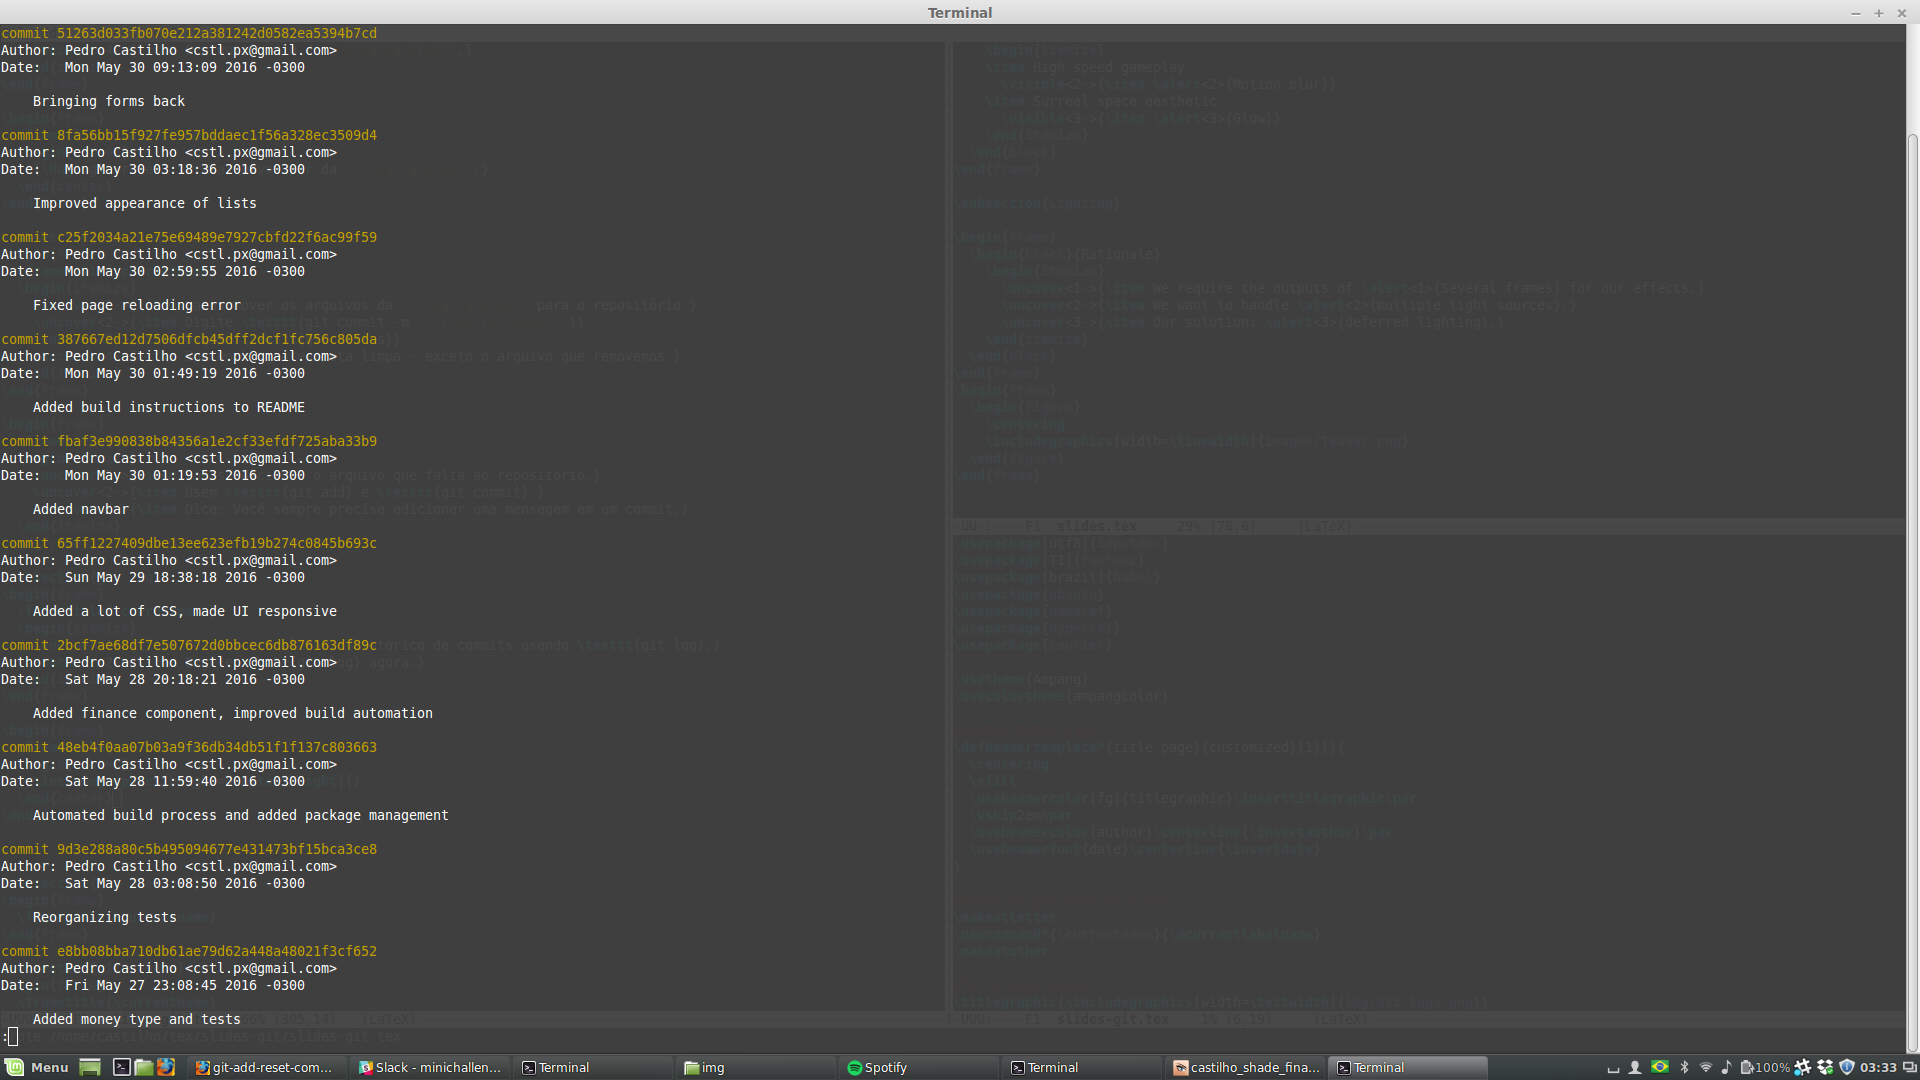
\includegraphics[height=0.8\textheight]{img/git-log.png}
  \end{center}
\end{frame}

\subsection{git log}
\begin{frame}
  \frametitle{\currentname}
  \begin{itemize}
    \uncover<1->{\item Podemos visualizar o histórico de commits usando \texttt{git log}.}
    \uncover<1->{\item Digite \texttt{git log} agora.}
    \uncover<2->{\item Digite \texttt{q} para sair da lista de commits.}
  \end{itemize}
\end{frame}

\begin{frame}
  \frametitle{\currentname}
  \begin{center}
    {\Huge git log: mostra o histórico de commits.}
  \end{center}
\end{frame}

\subsection{O que vimos até agora}
\begin{frame}
  \frametitle{\currentname}
  \begin{center}
    
\includegraphics[width=0.8\textwidth]{img/git-add-reset-commit.png}
  \end{center}
\end{frame}

\subsection{git checkout}
\begin{frame}
  \frametitle{\currentname}
  \begin{itemize}
    \uncover<1->{\item Modifique mais algum arquivo e dê commit na sua modificação.}
    \uncover<2->{\item Podemos recuperar qualquer versão antiga do arquivo.}
    \uncover<3->{\item Use \texttt{git log} novamente e encontre o ID do commit anterior.}
    \uncover<4->{\item Digite \texttt{git checkout id\_do\_commit nome\_do\_arquivo}}
    \uncover<5->{\item Digite \texttt{git status}}
  \end{itemize}
\end{frame}

\begin{frame}
  \frametitle{\currentname}
  \begin{itemize}
    \uncover<1->{\item \texttt{git checkout} também pode ser usado para retornar o projeto inteiro a um commit anterior.}
    \uncover<2->{\item Digite \texttt{git checkout id\_do\_commit}}
    \uncover<3->{\item Digite \texttt{git status}}
    \uncover<4->{\item Nossa ``Working Area'' agora está no estado de um commit antigo.}
    \uncover<5->{\item Nós podemos salvar esse estado, mas por enquanto vamos voltar ao commit anterior.}
    \uncover<6->{\item Digite \texttt{git checkout master}}
  \end{itemize}
\end{frame}

\begin{frame}
  \frametitle{\currentname}
  \begin{center}
    {\Huge git checkout: restaura versões antigas de arquivos ou do projeto inteiro. 
     \par\vskip2em HEAD: identificador especial que indica a versão do projeto que você está visualizando. 
    }
  \end{center}
\end{frame}

\begin{frame}
  \frametitle{\currentname}
  \begin{center}
    {\Huge master: nome padrão do git para a versão principal do projeto. 
    }
  \end{center}
\end{frame}

\begin{frame}
  \frametitle{\currentname}
  \begin{center}
    Uma última dica: \texttt{git checkout -{}- nome\_do\_arquivo} restaura o arquivo à versão dele no HEAD.
  \end{center}
\end{frame}

\subsection{O que vimos até agora}
\begin{frame}
  \frametitle{\currentname}
  \begin{center}
    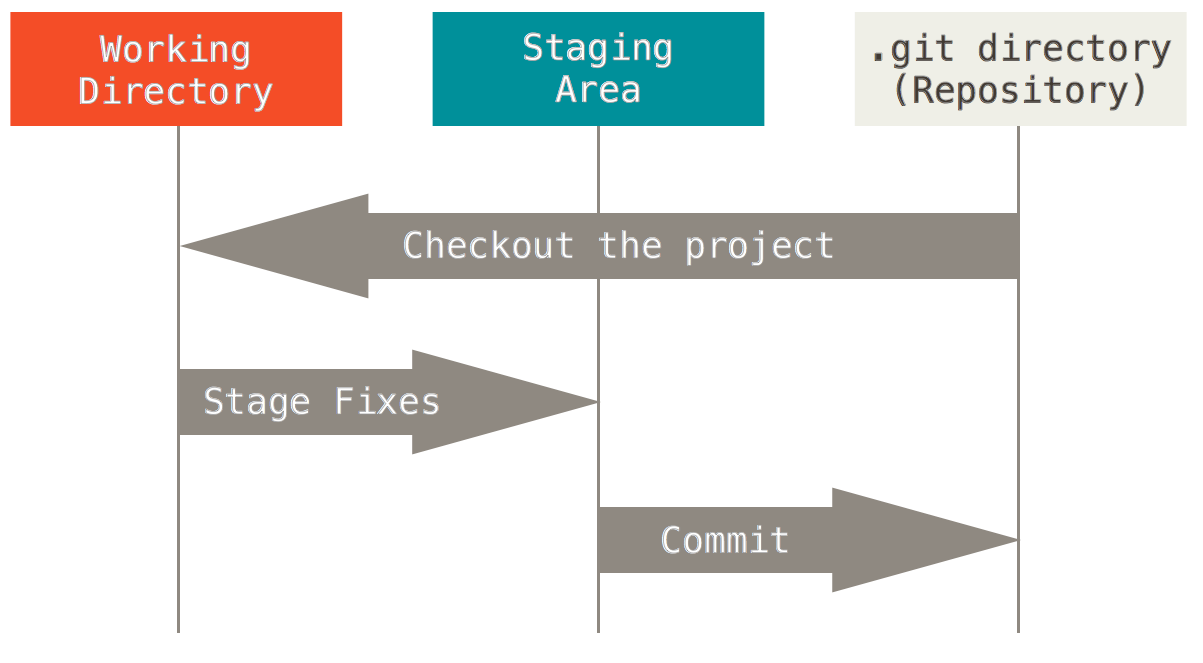
\includegraphics[width=0.8\textwidth]{img/areas.png}
  \end{center}
\end{frame}

\subsection{Quando tudo dá errado}
\begin{frame}
  \frametitle{\currentname}
  \begin{itemize}
    \uncover<1->{\item Fazer um commit toda vez que você faz alguma alteração relevante no projeto pode salvar sua vida.}
    \uncover<2->{\item Os seus commits são salvos \textbf{permanentemente}.}
    \uncover<3->{\item Caso no futuro algo dê errado, você pode simplesmente restaurar o projeto.}
  \end{itemize}
\end{frame}

\begin{frame}
  \begin{center}
    {\Huge Dúvidas?}
  \end{center}
\end{frame}

\section{Trabalhando com branches}

\subsection{git branch}
\begin{frame}
  \frametitle{\currentname}
  \begin{itemize}
    \uncover<1->{\item Às vezes queremos fazer modificações sem quebrar o que já temos pronto.}
    \uncover<2->{\item O git te permite criar um ``ramo'' de trabalho isolado do resto do projeto.}
    \uncover<3->{\item Digite \texttt{git branch}}
    \uncover<4->{\item Agora digite \texttt{git branch mybranch}}
    \uncover<5->{\item Digite \texttt{git branch} novamente.}
  \end{itemize}
\end{frame}


\begin{frame}
  \frametitle{\currentname}
  \begin{center}
    {\Huge git branch: lista branches existentes e cria branches novos.}
  \end{center}
\end{frame}


\subsection{git checkout (de novo)}
\begin{frame}
  \frametitle{\currentname}
  \begin{itemize}
    \uncover<2->{\item Vamos mudar para o branch que criamos.}
    \uncover<3->{\item Digite \texttt{git checkout mybranch}}
    \uncover<4->{\item Digite \texttt{git branch}}
    \uncover<5->{\item Modifique algum arquivo e dê commit}
    \uncover<6->{\item Digite \texttt{git checkout master}}
    \uncover<7->{\item As modificações são limitadas ao branch onde são feitas.}
  \end{itemize}
\end{frame}


\begin{frame}
  \frametitle{\currentname}
  \begin{center}
    {\Huge git checkout: também altera a versão do projeto para branches diferentes.}
  \end{center}
\end{frame}

\subsection{git merge}
\begin{frame}
  \frametitle{\currentname}
  \begin{itemize}
    \uncover<1->{\item Suponhamos que terminamos uma feature nova, e queremos integrá-la ao projeto principal.}
    \uncover<2->{\item Para isso, precisamos combinar 2 branches.}
    \uncover<3->{\item Modifique as mesmas linhas arquivo que você modificou no branch \texttt{mybranch}.}
    \uncover<4->{\item Digite \texttt{git merge mybranch}}
  \end{itemize}
\end{frame}

\subsection{Conflitos}
\begin{frame}
  \frametitle{\currentname}
  \begin{center}
    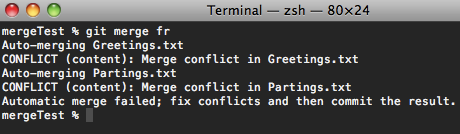
\includegraphics[width=0.8\textwidth]{img/conflict.png}
  \end{center}
\end{frame}

\begin{frame}
  \frametitle{\currentname}
  \begin{center}
    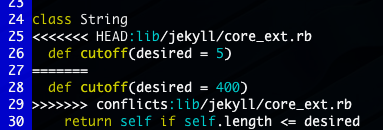
\includegraphics[width=0.8\textwidth]{img/conflicts.png}
  \end{center}
\end{frame}

\begin{frame}
  \frametitle{\currentname}
  \begin{itemize}
    \uncover<1->{\item Após resolver o conflito, comittem a versão com o conflito resolvido.}
    \uncover<2->{\item Digitem \texttt{git log}}
    \uncover<3->{\item O conflito fica salvo - você pode repetir a resolução do conflito se a anterior não for satisfatória.}
    \uncover<4->{\item Voltem para o conflito usando \texttt{git checkout}}
    \uncover<5->{\item Usem \texttt{git checkout -b novo\_branch} para criar um novo branch com o conflito}
    \uncover<6->{\item Resolvam o conflito de forma diferente no novo branch}
    \uncover<7->{\item Deem merge do novo branch com \texttt{master} e resolvam o conflito novamente}
  \end{itemize}
\end{frame}

\begin{frame}
  \frametitle{\currentname}
  \begin{center}
    {\Huge git merge: combina duas versões diferentes do projeto.}
  \end{center}
\end{frame}

\subsection{O que vimos até agora}
\begin{frame}
  \frametitle{\currentname}
  \begin{center}
    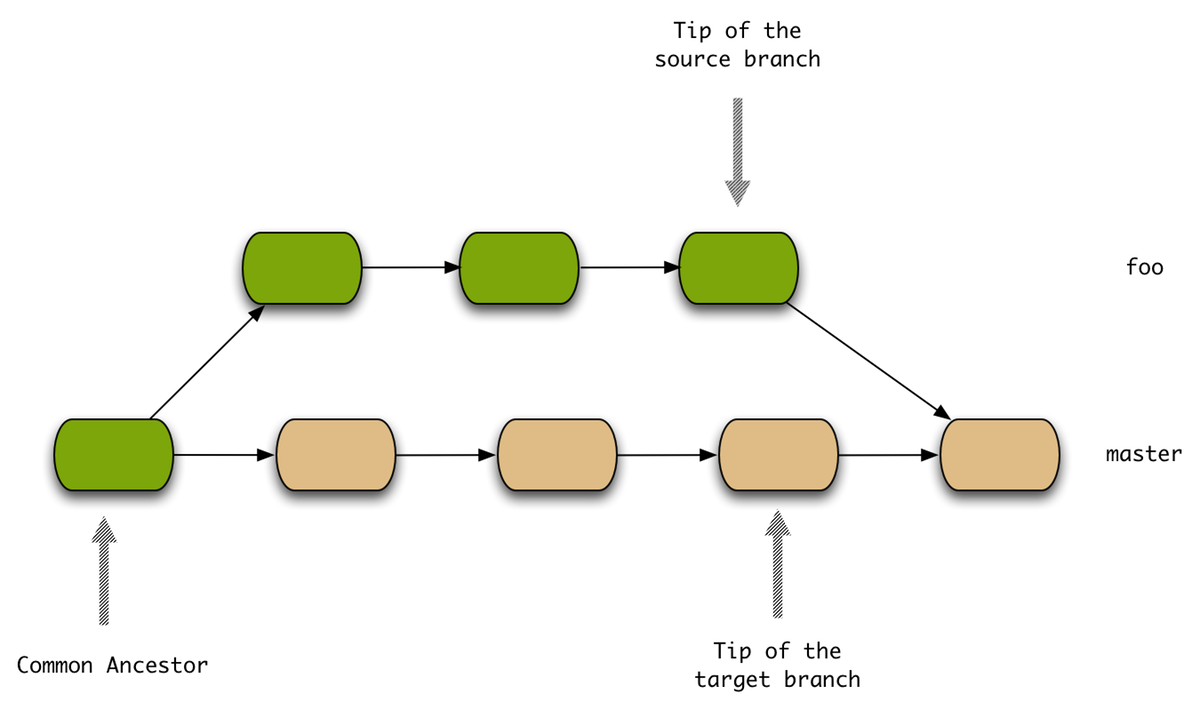
\includegraphics[width=0.8\textwidth]{img/git-merge.png}
  \end{center}
\end{frame}

\begin{frame}
  \begin{center}
    {\Huge Dúvidas?}
  \end{center}
\end{frame}

\section{Trabalhando com repositório remoto}
\subsection{Provedores de repositórios}
\begin{frame}
  \frametitle{\currentname}
  \begin{center}
    
\includegraphics[width=0.8\textwidth]{img/github-logo.png}
  \end{center}
\end{frame}

\begin{frame}
  \frametitle{\currentname}
  \begin{center}
    
\includegraphics[width=0.8\textwidth]{img/bitbucket-logo.png}
  \end{center}
\end{frame}

\subsection{git clone}
\begin{frame}
  \frametitle{\currentname}
  \begin{itemize}
    \uncover<1->{\item Vocês vão todos salvar uma cópia deste slide para terem como referência depois.}
    \uncover<2->{\item Vocês vão fazer isso usando o git!}
    \uncover<3->{\item Digitem \texttt{git clone https://github.com/pcstl/git-workshop.git}}
  \end{itemize}
\end{frame}

\begin{frame}
  \frametitle{\currentname}
  \begin{center}
    {\Huge git clone: copia código de repositórios remotos.}
  \end{center}
\end{frame}

\subsection{git remote}
\begin{frame}
  \frametitle{\currentname}
  \begin{itemize}
    \uncover<1->{\item Na pasta onde vocês baixaram os slides, digitem \texttt{git remote}}
    \uncover<2->{\item Vocês vão ver um link com o nome \texttt{origin}}
    \uncover<3->{\item Esse é um repositório \textit{remoto} ligado a seu projeto.}
    \uncover<4->{\item Você também pode adicionar repositórios remotos com \texttt{git remote add nome\_do\_repositório link\_do\_repositório}}
    \uncover<5->{\item Repositórios remotos podem ser usados para \textit{centralizar} o projeto.}
  \end{itemize}
\end{frame}

\subsection{git pull}
\begin{frame}
  \frametitle{\currentname}
  \begin{itemize}
    \uncover<1->{\item Suponhamos que um membro do seu time adicionou features novas ao repositório remoto e você quer pegar elas.}
    \uncover<2->{\item Para fazer isso, use \texttt{git pull nome\_do\_repositório nome\_do\_branch\_remoto}}
    \uncover<3->{\item Esse comando irá fazer um merge entre o branch em que você está e o branch que você escolheu no repositório remoto.}
    \uncover<4->{\item Conflitos podem ocorrer da mesma forma que em um merge normal.}
  \end{itemize}
\end{frame}

\subsection{git push}
\begin{frame}
  \frametitle{\currentname}
  \begin{itemize}
    \uncover<1->{\item O contrário do \texttt{git pull} é o \texttt{git push.}}
    \uncover<2->{\item Ele manda suas alterações para o repositório remoto.}
    \uncover<3->{\item Se o repositório estiver mais atualizado que sua versão, o push falha.}
    \uncover<4->{\item Para evitar isso, dê pull antes do push.}
    \uncover<5->{\item sintaxe: \texttt{git push nome\_do\_repositório nome\_do\_branch\_local}}
  \end{itemize}
\end{frame}

\begin{frame}
  \frametitle{\currentname}
  \begin{center}
    {\Huge git pull: puxa atualizações do repositório remoto para sua versão local. 
     \par\vskip2em git push: manda atualizações da sua versão local para o repositório remoto. 
    }
  \end{center}
\end{frame}

\subsection{O que vimos até agora}
\begin{frame}
  \frametitle{\currentname}
  \begin{center}
    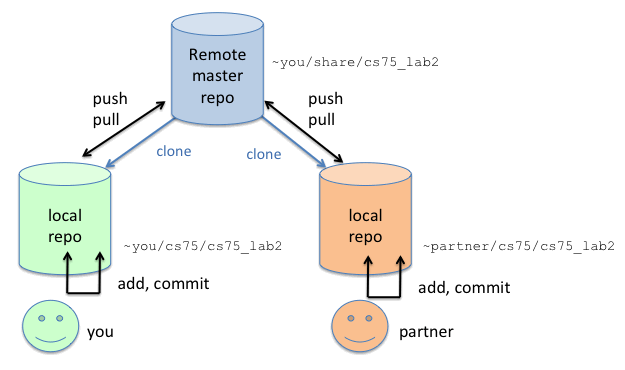
\includegraphics[width=0.8\textwidth]{img/gitrepos.png}
  \end{center}
\end{frame}

\begin{frame}
  \begin{center}
    {\Huge Dúvidas?}
  \end{center}
\end{frame}

\section{Colaboração}
\subsection{Fluxo de trabalho}
\begin{frame}
  \frametitle{\currentname}
  \begin{itemize}
    \uncover<1->{\item O ideal é que pessoas diferentes do grupo trabalhem em coisas diferentes para evitar conflitos.}
    \uncover<2->{\item Mantenham a versão ``oficial'' no repositório remoto - assim, se der merda, vocês sempre podem puxar de lá.}
    \uncover<3->{\item Nunca mandem código que não funciona para o remoto - trabalhem localmente até funcionar.}
    \uncover<4->{\item Desenvolvam features diferentes em branches separados - só deem merge quando a feature estiver pronta.}
    \uncover<5->{\item Em último caso, checkout na última versão que funcionava!}
  \end{itemize}
\end{frame}

\section{Interfaces gráficas}
\subsection{GitKraken}
\begin{frame}
  \frametitle{\currentname}
  \begin{center}
    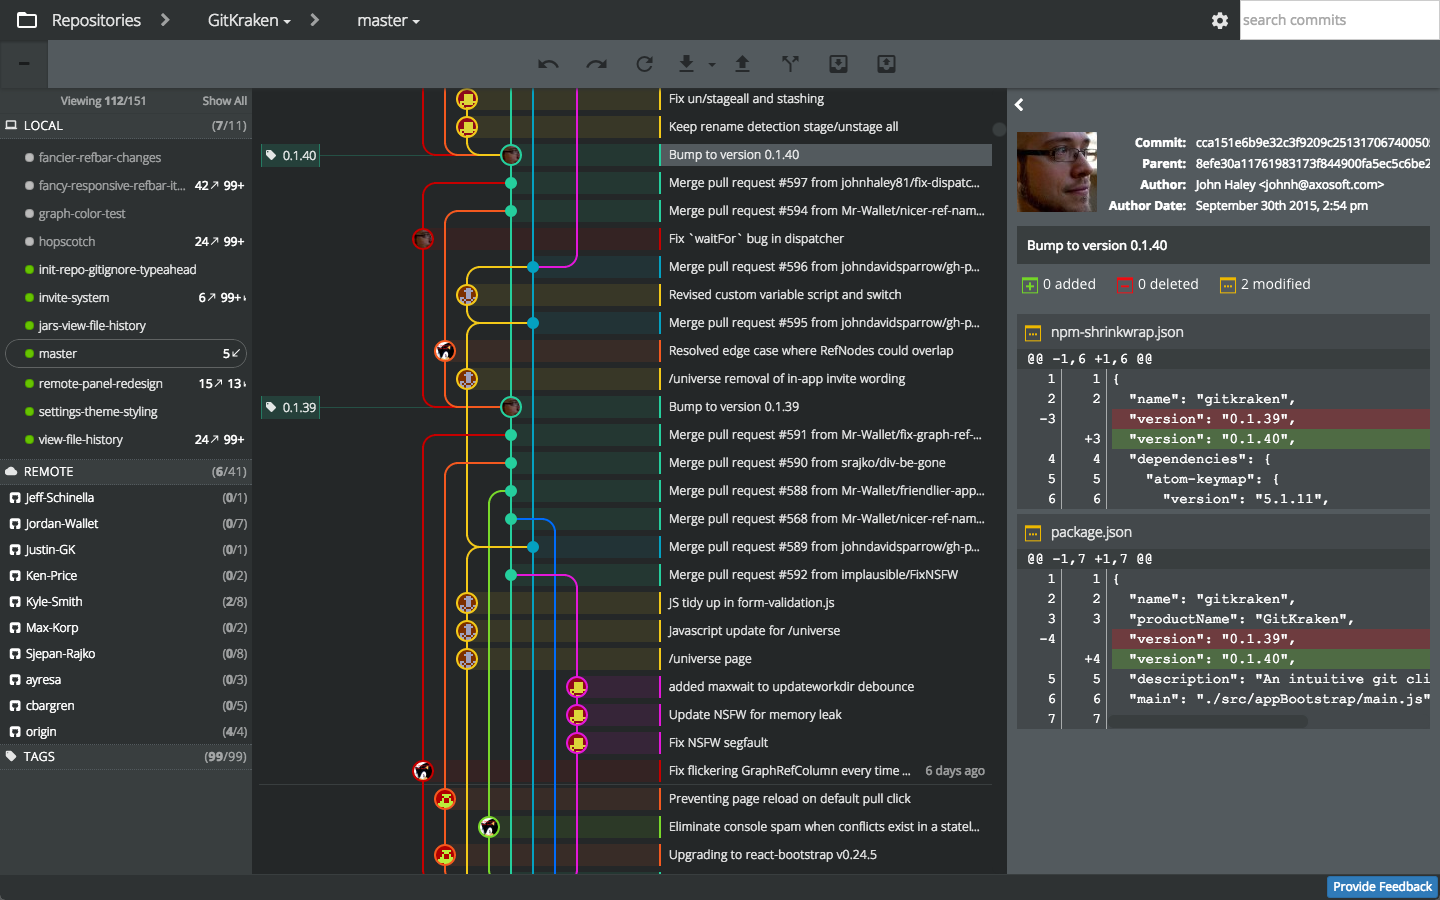
\includegraphics[height=0.6\textheight]{img/gitkraken.png}
  \end{center}
\end{frame}

\subsection{Github Desktop}
\begin{frame}
  \frametitle{\currentname}
  \begin{center}
    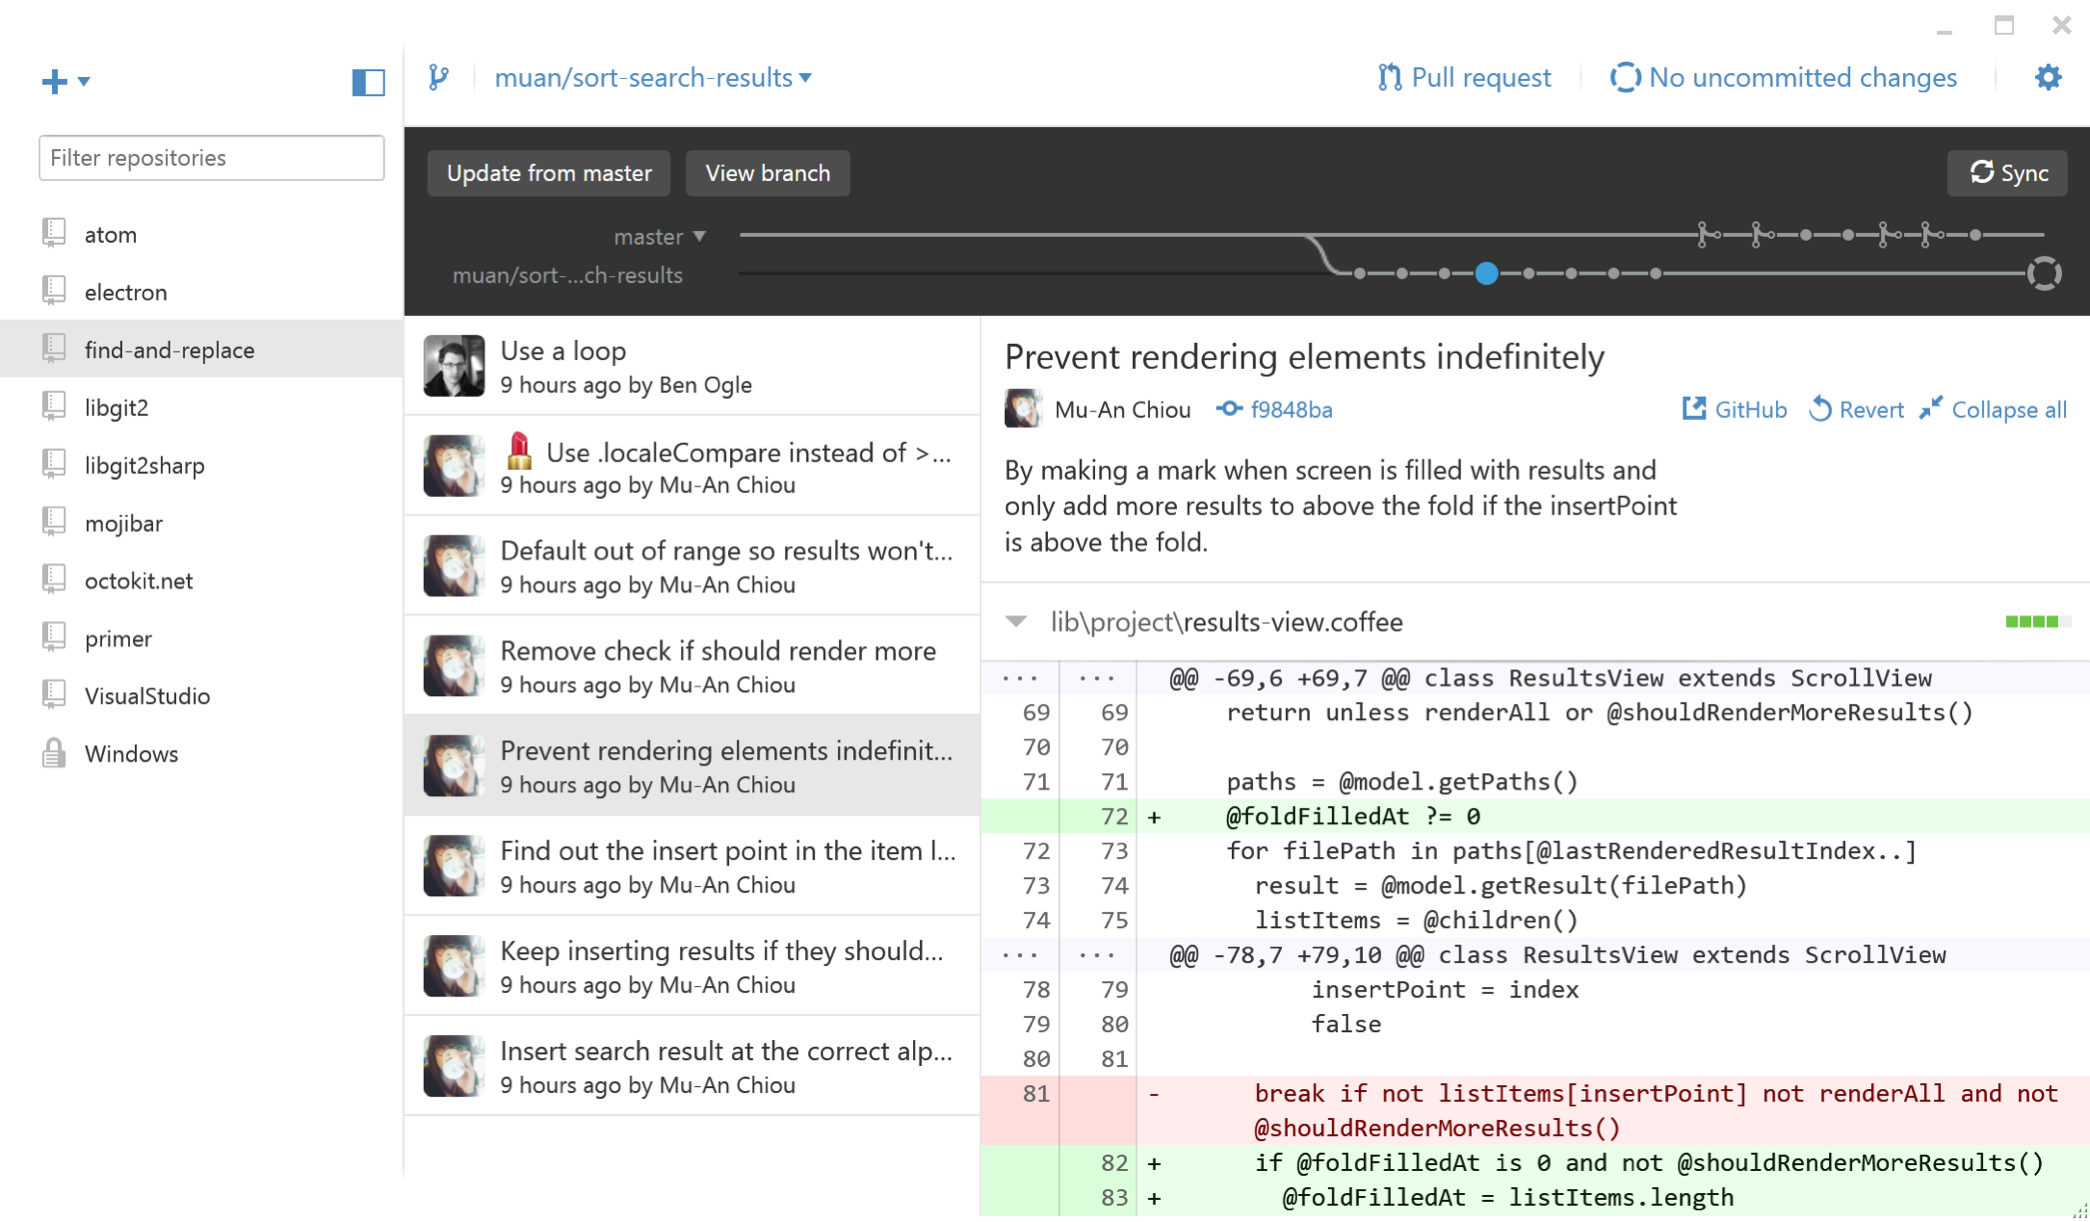
\includegraphics[height=0.6\textheight]{img/github-desktop.png}
  \end{center}
\end{frame}

\section{Buscando ajuda}
\subsection{Sites úteis}
\begin{frame}
  \frametitle{\currentname}
  \begin{itemize}
    \item Documentação oficial do git $\rightarrow$ \href{https://git-scm.com/documentation}{https://git-scm.com/documentation}
    \item Tutoriais do GitHub $\rightarrow$ \href{https://guides.github.com/}{https://guides.github.com/}
    \item Tutoriais da Atlassian $\rightarrow$ \href{https://www.atlassian.com/git/tutorials/}{https://www.atlassian.com/git/tutorials/}
  \end{itemize}
\end{frame}

\begin{frame}
  \begin{center}
    {\Huge Dúvidas?}
  \end{center}
\end{frame}

\end{document}

